% !TEX encoding = UTF-8 Unicode
% !TEX root = ../rapport.tex

\chapter{Introduction}\label{intro}


Les réseaux sans fil font depuis plus d'une dizaine d'années partie intégrante de la vie quotidienne des entreprises, des particuliers, de l'industrie et d'autres organisations. Ils
représentent aujourd'hui une des briques de base sur lesquelles vont se fonder les systèmes
intelligents omniprésents qui vont constituer une des technologies de l'avenir. Cependant, la majeure partie de ces technologies sans fils, à commencer par le Wifi, elle est basée  sur des infrastructures fixes, limitant la mobilité des utilisateurs. Pour faciliter cette mobilité, il existe  un autre type de réseau, de plus en plus courant, qui  permet aux nœuds du réseau de communiquer directement entre eux sans nécessiter d’infrastructure : ce sont les réseaux ad hoc.

\begin{figure}[h]
\centering
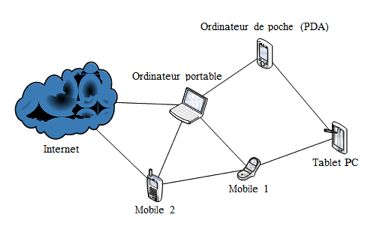
\includegraphics[scale=0.8]{Intro/reseauAdHoc.png}
\caption{\label{reseauAdHoc} Exemple de réseau ad hoc}
\end{figure}

On distingue donc deux principales classes de réseaux sans fils, les classiques structurés et les non structurés comme les réseaux ad hoc. Les réseaux ad hoc offrent la possibilité de connecter différents dispositifs sans avoir à préinstaller une infrastructure fixe comme dans les réseaux traditionnels. Dans les réseaux ad hoc, l’ensemble des nœuds communiquent directement entre eux (voir figure \ref{reseauAdHoc}). Nous allons nous intéresser à un type particulier de réseau ad hoc :  les réseaux de capteurs. Ces réseaux ont de nombreuses applications pratiques dans le médicale, la physique, la chimie, le multimédia, l'automobile, la climatologie…



\section{Capteurs}

Les capteurs sont des petites entités électroniques à faible coût qui ont pour but de récolter des informations dans leur environnement proche comme la température, la vitesse, le bruit, la pression, le mouvement, la chaleur ou la lumière… La valeur mesurée est convertie dans une représentation analogique ou numérique.

\begin{figure}[h]
\centering
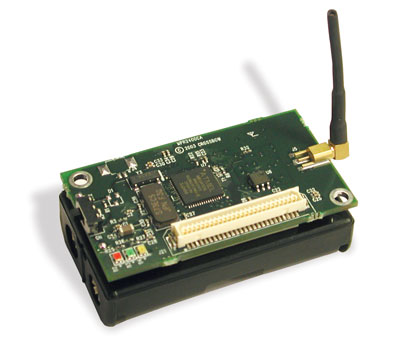
\includegraphics[scale=0.4]{Intro/imageCapteur}
\caption{\label{imageCapteur} Capteur sans fil}
\end{figure}

Il existe des \textbf{capteurs intelligents} (Smart Sensors) dans lesquels coexistent le(s) capteur(s) et les circuits de traitement et de communication. Leurs relations avec des couches de traitement supérieures vont bien au-delà d’une simple « transduction de signal ». Les capteurs intelligents sont des « capteurs d’informations » et non pas simplement des capteurs et des circuits de traitement du signal juxtaposés. De plus, les « Smart Sensors » ne sont pas des dispositifs banalisés car chacun de leurs constituants a été conçu dans l’objectif d’une application bien spécifique.

Lorsque nous parlerons de capteur plus loin dans ce rapport, il s'agira d'un capteur intelligent. Un tel capteur contient quatre unités de base (voir Figure \ref{archiCapteur}) : 
 
 \begin{figure}[h]
\centering

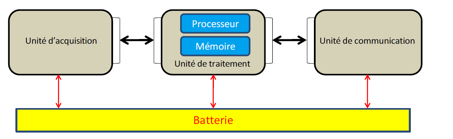
\includegraphics[scale=0.6]{Intro/archiCapteur}
\caption{\label{archiCapteur} Architecture d’un capteur}
\end{figure}
 
 \begin{description}
\item[L'unité d’acquisition] est composée d’un capteur qui obtient des mesures sur les paramètres environnementaux et d’un convertisseur Analogique/Numérique qui convertit l’information relevée et la transmet à l’unité de traitement. La perception d'un capteur est limitée par un rayon de sensation (Rs). La  Figure \ref{percept} illustre ce principe.

\item[L'unité de traitement] est composée d’un processeur et d’une mémoire intégrant un système d’exploitation spécifique. Cette unité possède deux interfaces, une interface pour l’unité d’acquisition et une interface pour l’unité de communication. Elle acquiert les informations en provenance de l’unité d’acquisition et les envoie à l’unité de communication. Cette unité est chargée aussi d’exécuter les protocoles de communications qui permettent de faire collaborer le capteur avec d’autres capteurs. Elle peut aussi analyser les données captées.

\item[L'unité de communication] est l'unité responsable de toutes les émissions et réceptions de données via un support de communication radio. Elle peut être de type optique, ou de type radiofréquence. Fonctionnellement chaque capteur possède un rayon de communication (Rc). La  figure \ref{percept} montre la zone dans laquelle le capteur peut communiquer. Certains capteurs peuvent moduler leur rayon de communication.

\item[L'unité de contrôle d'énergie (batterie)] sert à alimenter tous les composants. Cependant, à cause de la taille réduite du capteur, la batterie est limitée et généralement irremplaçable. Ainsi, l’énergie est la ressource la plus précieuse puisqu’elle influe directement sur la durée de vie des capteurs.
\end{description}

Selon son domaine d'application, un capteur peut contenir des modules supplémentaires comme le système de positionnement GPS (Global Positioning System) ou un système lui permettant de se déplacer.

\begin{figure}[h]
\centering
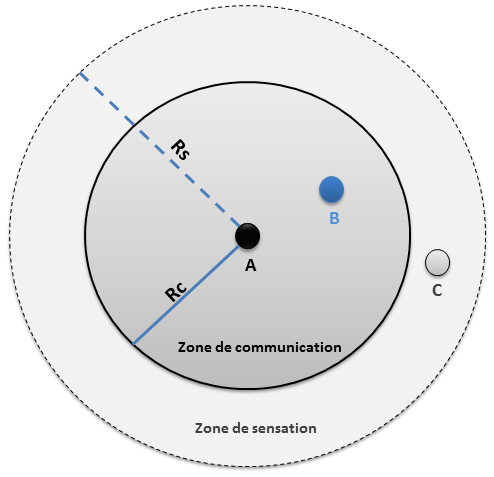
\includegraphics[scale=0.7]{Intro/percept}
\caption{\label{percept} Rayon de communication et de sensation}
\end{figure}




\section{Caractéristiques techniques des capteurs actuels}

\begin{description}
\item[Une faible puissance de calcul] : quand les ordinateurs peuvent avoir jusqu'à 4 processeurs, chacun cadencé à 3GHz, ou quand les derniers Smartphones peuvent fonctionner jusqu’à 800MHz, un capteur actuel est à peine plus puissant qu’une calculatrice graphique produite dans les années 90.

\item[Un espace de stockage mémoire limité] à quelques kilo-octets ou quelques méga-octets impose l'utilisation d'algorithmes distribués, localisés et collaboratifs.

\item[Une puissance radio limitée] : l’ordre de grandeur des portées actuellement atteignables par les principaux capteurs est d’une centaine de mètres en extérieur et de quelques dizaines de mètres en intérieur. Cette portée est largement dépendante de la fréquence utilisée et de l’environnement. Elle nécessite un routage multi-saut pour l’acheminement des données vers une entité de collecte : le puits. Les capteurs ne peuvent communiquer qu’avec leur voisinage direct qui va relayer les communications.

\item[Un débit faible] : les composants radio d’un capteur sont limités à quelques centaines de kilo-octets par seconde.

\item[Une réserve d’énergie réduite] : même s’il existe des mécanismes de recharge d’énergie, la durée de vie d’un capteur reste directement liée au niveau de sa batterie. Cette réserve d’énergie est partagée par chaque unité d’un capteur mais l’unité de communication va en consommer près de 95\% lors du fonctionnement actif du capteur. Les enjeux actuels portent donc sur :
	\begin{itemize}
	\item l’augmentation des capacités des batteries
	\item les dispositifs de transmission radio ultra-basse consommation
	\item les architectures basse consommation
	\item des mécanismes d’endormissement
	\item des protocoles de communication spécifiques
	\end{itemize}
\end{description}



\section{Réseau de capteurs sans fil (Wireless Sensors Network)}
Les réseaux de capteurs sans fil sont un type particulier de réseau ad-hoc. Ces réseaux sont formés d’une multitude de capteurs, capables de s’auto-organiser et ainsi de travailler pour la collecte, le partage et le traitement coopératif des informations sur leur environnement ; le tout sans intervention humaine. Ces dispositifs sont peu coûteux, mais peu performants. Depuis quelques décennies, le besoin croissant d’observer et de contrôler des phénomènes physiques tels que la température, la pression ou encore la luminosité a conduit au déploiement de nombreux réseaux de capteurs.

\begin{figure}[h]
\centering
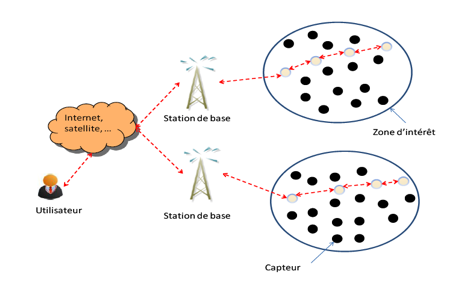
\includegraphics[scale=0.8]{Intro/WSN}
\caption{\label{WSN} Réseaux de capteurs}
\end{figure}

Dans l'exemple de la figure \ref{WSN}, les capteurs sont déployés d’une manière aléatoire dans une zone d’intérêt, et une station de base, située à l’extrémité de cette zone, est chargée de récupérer les données collectées par les capteurs. Lorsqu’un capteur détecte un événement pertinent, un message d’alerte est envoyé à la station de base par le biais d’une  communication entre les capteurs. Les données collectées sont traitées et analysées par des machines puissantes.



\subsection{Architecture}



\begin{figure}[h]
\centering
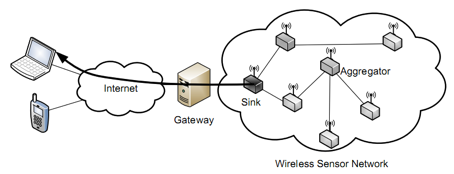
\includegraphics[scale=0.8]{Intro/archiWSN}
\caption{\label{archiWSN} architecture d’un réseau WSN}
\end{figure}

Les réseaux de capteurs sans fils sont construits autour des quatre principales entités suivantes :

\begin{description}
\item[Les capteurs] décrits précédemment.

\item[L’agrégateur] est en charge d’agréger les messages qu’il reçoit de plusieurs capteurs puis de les envoyer en un seul message au puits. Cette opération a pour principal but de limiter le trafic sur le réseau et donc de prolonger la durée de vie globale du réseau de capteur.

\item[Le puits] est le nœud final  du réseau. C’est à lui qu’est  envoyé l’ensemble des valeurs mesurées par le réseau.  Il peut arriver qu’il y ait plusieurs puits sur un même réseau de capteurs.

\item[La passerelle] est un dispositif qui a la particularité d’avoir deux interfaces réseau. Elle permet de relier le réseau de capteurs  sans fils  à un réseau plus traditionnel, typiquement l’internet. Habituellement  le réseau de capteurs  ne sert  qu’à  faire remonter les 
mesures, les applications traitant ces informations étant exécutées sur la machine 
de l’utilisateur final.
\end{description}



\subsection{Caractéristiques}

\begin{description}
\item[L'absence d’infrastructure] préexistante et de tout genre d’administration centralisée.

\item[Des interférences] : les liens radio ne sont pas isolés, deux transmissions simultanées sur une même fréquence, ou utilisant des fréquences proches, peuvent interférer.

\item[Une taille importante] : un réseau de capteurs peut contenir des milliers de nœuds.

\item[L'hétérogénéité des nœuds] : plusieurs types de capteurs différents connectés entre eux.


\item[Une topologie dynamique] : les capteurs peuvent être attachés à des objets mobiles qui se déplacent d’une façon libre et arbitraire rendant ainsi la topologie du réseau fréquemment changeante.

\item[Des contraintes énergétiques] : la caractéristique la plus critique dans les réseaux de capteurs est la modestie de ses ressources énergétiques (batterie).

\item[La capacité de stockage et la puissance de calcul] sont limitées dans un capteur.

\item[Une bande passante limitée] en raison des caractéristiques techniques des radios.

\item[Le faible coût du matériel] qui facilite une redondance des liens pour assurer une connexité du réseau en cas de panne d’un ou plusieurs capteurs.

\item[L’impossibilité de remplacer manuellement les nœuds] dans le cas où leur position est inconnue (déploiement rapide dans des conditions difficiles ; absence de puce GPS…).

\item[Le caractère aléatoire de la topologie du réseau] : celui-ci est déployé en fonction des zones d'intérêt ou aléatoirement.
\end{description}



\subsection{Problématique et défis}

Les caractéristiques particulières des réseaux de capteurs modifient les critères de performance par rapport aux réseaux sans fil traditionnels. Dans les réseaux locaux filaires ou les réseaux cellulaires, les critères les plus pertinents sont le débit, la latence et la qualité de service. En effet, les nouvelles activités telles que le transfert d’images,  le  transfert de vidéos, et la navigation sur Internet requièrent de bonnes performances selon ces trois critères.

En revanche, dans les réseaux de capteurs conçus pour surveiller une zone d’intérêt,  la longévité du réseau est fondamentale. De ce fait, la conservation de l’énergie est devenue un critère de performance prépondérant et se pose en premier lieu tandis que les autres critères comme le débit ou l’utilisation de la bande passante sont devenus secondaires.

Les perspectives d’application des réseaux de capteurs sont enthousiasmantes mais les défis qu’elles posent n’en sont pas moins nombreux et complexes. Parmi les problématiques cruciales, nous pouvons citer :

\begin{description}
\item[L’énergie] : cette contrainte impose de concevoir des protocoles économes en énergie.

\item[Le routage] : le problème de routage consiste à déterminer un acheminement optimal des paquets à travers le réseau au sens d’un certain critère de performance (l'énergie par exemple).

\item[La sécurité] : la puissance de calcul limitée d’un capteur ouvre de véritables défis pour concevoir des algorithmes de cryptages distribués et des politiques de confiance spécifiques.

\item[La collecte de données] : récupérer les données des capteurs et les assembler.

\item[L'auto-configuration] : une partie des applications visées appartient au domaine des applications domestiques. Il est donc important que le routage, l’intégration et l’adaptation à l’environnement soient transparents pour l’utilisateur.

\item[L'autoréparation] : les capteurs sont parfois inaccessibles (intégrés dans un mur, installés chez un particulier, déployés dans une zone dangereuse, etc.) et de conception peu sûre (faible coût de production). Une solution complète doit donc gérer efficacement la perte ou l’ajout d’un nœud dans le réseau.

\item[La localisation] : il s’agit de concevoir des mécanismes de localisation réalistes vis-à-vis des contraintes et des applications propres aux réseaux de capteurs. Les solutions actuellement proposées sont soit imprécises, soit coûteuses en énergie ou en matériel.
\end{description}

Dans la section \ref{etat_art}, nous ferons un état de l'art des algorithmes de routage dans les réseaux de capteur sans fil. Puis en section \ref{Analyse_et_reflexion}, nous établirons un modèle et analyserons quelques algorithmes existants. En section \ref{simu}, nous présenterons des résultats de simulations sur la plateforme WSNET. Enfin nous conclurons ce rapport.


